\documentclass[twoside,a4paper,10pt]{report}
%%\usepackage[french]{babel} %% Use your own babel language
\usepackage[top=3cm,bottom=3cm,left=2.5cm,right=2.5cm]{geometry}
%\usepackage{ucs}
\usepackage[utf8]{inputenc}
\usepackage{pslatex}
\usepackage{hyperref}
\usepackage{graphicx}
\usepackage{tabularx}
\usepackage{supertabular}
\usepackage{pdflscape} %% Used for very big table
\usepackage{moreverb}
\usepackage{color}
\usepackage{listings}
\usepackage{lastpage}
\usepackage{fancyhdr}
\usepackage{ulem}
\usepackage{textcomp}
\usepackage{wasysym}
\usepackage{wrapfig} %%Usefull for image 
%\usepackage{fguill} %%Use this package for guillemot[left|right] useless with babel set to french
\usepackage{eso-pic} %% Background

\usepackage{sectsty} %%Change style on every sections\pagestyle{fancy}%
\renewcommand{\headrulewidth}{0.1pt}
\renewcommand{\footrulewidth}{0pt}
\renewcommand{\chaptermark}[1]{%
	\markboth{\chaptername\ \thechapter.\ #1}{}}

\renewcommand{\sectionmark}[1]{%
	\markright{#1}{}}

\fancypagestyle{plain}{%
\fancyhf{}
\fancyfoot[R]{\thepage/\pageref{LastPage}}
\renewcommand{\headrulewidth}{0pt}
\renewcommand{\footrulewidth}{0pt}}
\fancyhf{}
\fancyhead[L]{\rightmark}
\fancyhead[R]{\leftmark}
\fancyfoot[R]{\thepage/\pageref{LastPage}}
\renewcommand{\headrulewidth}{0.1pt}
\renewcommand{\footrulewidth}{0pt}

\definecolor{codegray}{gray}{.95}
\lstset{language=C,
	numbers=left,
	tabsize=2,
	basicstyle=\scriptsize,
	stringstyle=\textrm,
	showstringspaces=false,
	frame=none,
	xleftmargin=3pt,
	backgroundcolor=\color{codegray}}

\newcommand{\settexitref}[2]{(\ref{#1}p\pageref{#1})}
%\newcommand{\dokutitlelevelone}[1]{\chapter{#1}}
\newcommand{\dokutitlelevelone}[1]{} %ignore the level one, which is the page title
%\newcommand{\dokutitleleveltwo}[1]{\section{#1}}
\newcommand{\dokutitleleveltwo}[1]{\chapter{#1}}
%\newcommand{\dokutitleleveltree}[1]{\subsection{#1}}
\newcommand{\dokutitleleveltree}[1]{\section{#1}}
%\newcommand{\dokutitlelevelfour}[1]{\subsubsection{#1}}
\newcommand{\dokutitlelevelfour}[1]{\subsection{#1}}
\newcommand{\dokutitlelevelfive}[1]{\paragraph{#1}}
\newcommand{\dokufootnote}[1]{\footnote{#1}}
\newcommand{\dokufootmark}[1]{\footnotemark[#1]}
\newcommand{\dokubold}[1]{\textbf{#1}}
\newcommand{\dokuitalic}[1]{\textsl{#1}}
\newcommand{\dokumonospace}[1]{\texttt{#1}}
\newcommand{\dokuunderline}[1]{\underline{#1}}
\newcommand{\dokuoverline}[1]{\sout{#1}}
\newcommand{\dokusupscript}[1]{\textsuperscript{#1}}
\newcommand{\dokusubscript}[1]{$_{#1}$}
\newcommand{\dokuhline}{\line(1,0){400}}
\newcommand{\dokulabel}[1]{\label{#1}}
\newcommand{\dokuitem}{\item}
\newcommand{\dokuquoting}{\textbar}
\newcommand{\dokutabularwidth}{\textwidth}
\newcommand{\dokusupertabularheadbreak}{\small\sl continued from previous page}
\newcommand{\dokusupertabulartailbreak}{\small\sl continued on next page}
\newcommand{\dokuheadingstyle}[1]{\textbf{#1}}
\definecolor{dokuheadingcolor}{rgb}{0,0,0.60}
\newcommand{\dokubackground}[1]{%
%\AddToShipoutPicture{%
%  \AtTextCenter{%
%    \makebox(0,0)[c]{\resizebox{\textwidth}{!}{%
%      \rotatebox{25}{\textsf{\textbf{\textcolor[gray]{0.90}{#1}}}}}}%
%  }%
% }%
}

\hypersetup{
pdftitle = { Dialogs: Grounding verbal interaction for robotics},
pdfauthor = {Patrick Tsemengue, Mahdi Chouayakh},
pdfcreator = {DokuTeXit},
pdfproducer = {dokuwiki + TeXit + latex + dvipdf}
}
\title{ Dialogs: Grounding verbal interaction for robotics}
\author{Patrick Tsemengue, Mahdi Chouayakh}
\dokubackground{http://homepages.laas.fr/slemaign/wiki/}
\begin{document}

\sffamily
\allsectionsfont{\sffamily}

\thispagestyle{empty}
\maketitle
\thispagestyle{empty}
\cleardoublepage
\tableofcontents
\newpage
\thispagestyle{plain}
\cleardoublepage
\newpage



\dokutitlelevelone{Conception map}
\label{bc34ce150ff26ff0ec4b6be60dcf178c}%% conception_map
\label{f0e926ab940662bebfe368ba24960a2d}%%Start: stage_natural_language_processing_-_ete_2010 => /home/slemaign/wiki/data/pages/stage_natural_language_processing_-_ete_2010.txt

\hyperref[d82c279ed6fd93ff2155ed19c4d2e7da]{Dialogs Module Simple Conception}

\begin{figure*}[h]
\centering
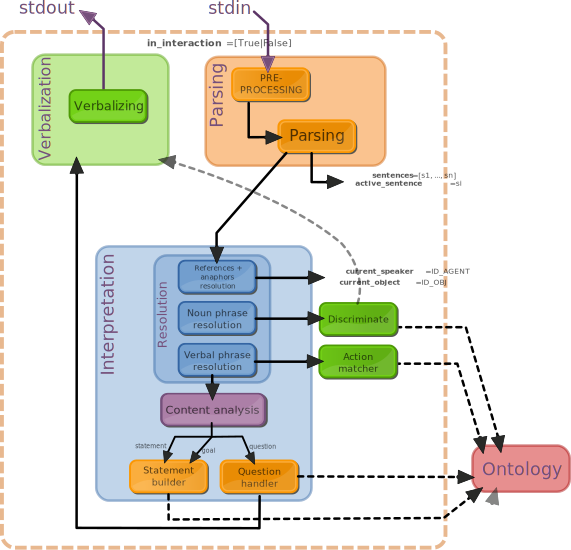
\includegraphics[width=\linewidth]{dialog_module_simple.png}
\caption{Dialogs overview}
\end{figure*}



\dokutitlelevelone{Data Structure}
\label{c8f6850ec2ec3fb32f203c1f4e3c2fd2}%% data_structure

\dokutitleleveltwo{Description}
\label{67daf92c833c41c95db874e18fcb2786}%% description

\begin{figure*}[h]
\centering
\includegraphics[width=\linewidth]{data_structs.png}
\caption{Data structures in Dialogs}
\end{figure*}


The \dokuitalic{Sentence data structure} consists of a tree of Nominal and verbal structures and \dokuitalic{Sentences}. The use of a tree eases the information fetching.
Inner components of a \dokuitalic{Sentence} are arranged into list of objects. Therefore, the data that is transmitted through the Dialogs modules will be a list of several \dokuitalic{Sentences}.


\begin{itemize}
\dokuitem  \dokuunderline{A Sentence is made of:}
\begin{itemize}
\dokuitem  \dokumonospace{sn}: a nominal structure typed into a list of Nominal{\textunderscore}group
\dokuitem  \dokumonospace{sv}: a verbal structure typed into a list of Verbal{\textunderscore}Group
\dokuitem  \dokumonospace{aim}: used for retrieving the purpose of a question (Mandatory when processing a w{\textunderscore}question or a subsentence)
\dokuitem  \dokumonospace{data{\textunderscore}type}: is the type of the sentence (w{\textunderscore}question, statement\ldots{})
\end{itemize}

\end{itemize}

\begin{itemize}
\dokuitem  \dokuunderline{Nominal group class declaration}
\begin{itemize}
\dokuitem  ‘‘det’’: determiner
\dokuitem  \dokumonospace{noun}: a simple noun
\dokuitem  \dokumonospace{adj}: a list of adjectives describing the noun
\dokuitem  \dokumonospace{noun{\textunderscore}cmpl}: the noun complements attribute, which is a list of Nominal{\textunderscore}group
\dokuitem  \dokumonospace{relative}: The relative subordinate clause, which is of a list of Sentences type
\end{itemize}

\end{itemize}

Additional Nominal Group attribute are:


\begin{itemize}
\dokuitem  ‘‘id’’: Holding the ontology identifier of its container nominal group set by default to none.
\dokuitem  \dokumonospace{{\textunderscore}resolved}: This hold the value TRUE when the Nominal group has been resolved (Cf. \hyperref[b7e164b34ff76b1cda93a058604190da]{Resolution})
\dokuitem  \dokumonospace{{\textunderscore}conjunction = 'AND' \#could be 'AND' or 'OR' }\ldots{} 
\dokuitem  \dokumonospace{ {\textunderscore}quantifier = 'ONE' \#could be 'ONE' or 'SOME' }\ldots{} (Cf. \hyperref[c9a5eb8d391a77a428b429e98ad45e2c]{Quantifier})
\end{itemize}

\begin{itemize}
\dokuitem  An indirect complement or adverbial is made of: 
\begin{itemize}
\dokuitem  Indirect complement class declaration
\dokuitem  \dokumonospace{gn}: nominal group
\dokuitem  \dokumonospace{prep}: preposition
\end{itemize}

\end{itemize}

\begin{itemize}
\dokuitem  \dokuunderline{Verbal group class declaration}
\begin{itemize}
\dokuitem  \dokumonospace{vrb{\textunderscore}main}: the main verb of a sentence
\dokuitem  \dokumonospace{vrb{\textunderscore}sec}: an accompanying verb of the main verb
\dokuitem  \dokumonospace{vrb{\textunderscore}tense}: the main verb tense
\dokuitem  \dokumonospace{d{\textunderscore}obj}: the direct object referred by the main verb
\dokuitem  \dokumonospace{i{\textunderscore}cmpl}: the indirect object referred by the main verb or an adverbial formed from a nominal group
\dokuitem  \dokumonospace{vrb{\textunderscore}adv}: an adverb describing the verb
\dokuitem  \dokumonospace{advrb}: an adverb used as an adverbial of the whole sentence
\dokuitem  ‘‘comparator’’: {the nominal group, object of the comparison}. Used for comparing nominal groups grammatically (E.g.: Bigger than)
\end{itemize}

\end{itemize}

\dokutitleleveltwo{Examples}
\label{bfebe34154a0dfd9fc7b447fc9ed74e9}%% examples
Input:


\small
\begin{verbatimtab}
The man, who talks now, has a new car
\end{verbatimtab}
\normalsize

Parsing result:


\small
\begin{verbatimtab}
  Sentence(Sentence.statement, '', 
      [Nominal_Group(['the'], ['man'], [], [],[Sentence(Sentence.relative, 'who', 
          [],  
          [Verbal_Group(['talk'],[],'present simple', 
              [], 
              [],
              [], ['now'] ,Verbal_Group.affirmative,[])])])],  
      [Verbal_Group(['have'], [],'present simple', 
          [Nominal_Group(['a'],['car'],[['new',[]]],[],[])],
          [],
          [], [] ,Verbal_Group.affirmative,[])])
\end{verbatimtab}
\normalsize

Input:


\small
\begin{verbatimtab}
I have played foot since I was a very young boy.
\end{verbatimtab}
\normalsize
Result:


\small
\begin{verbatimtab}
  Sentence(Sentence.statement, '', 
      [Nominal_Group([],['I'],[],[],[])], 
      [Verbal_Group(['play'], [],'present perfect', 
          [Nominal_Group(['a'],['foot'],[],[],[])], 
          [],
          [], [] ,Verbal_Group.affirmative,[Sentence('subsentence+statement', 'since', 
              [Nominal_Group([],['I'],[],[],[])], 
              [Verbal_Group(['be'], [],'past simple', 
                  [Nominal_Group(['a'],['boy'],[['young',['very']]],[],[])], 
                  [],
                  [], [] ,Verbal_Group.affirmative,[])])])])
\end{verbatimtab}
\normalsize

\dokutitlelevelone{Natural Language Parsing}
\label{40b6d909561b858c733e07e5b7595576}%% natural_language_parsing
We decided to store different data, with different functionalities in the sentence, in the same variable. The goal is to limit the data structure attribute number.
For example, we have decided to create a variable that contains the direct object of the verb and another one contains indirect complements of the verbs - indirect objects or adverbials that are noun phrases as both follow preposition.
Before starting the Parsing of the utterance, we attempt to give it a formalized form that eases the parsing. The following describe functions involved in the formalization process.


\dokutitleleveltwo{Pre-processing}
\label{786dd9bb7bc5625a566d42a2962bebf7}%% pre-processing

\dokutitleleveltree{Punctuation}
\label{9ac6d441030eb0844ffb83ba4f100c94}%% punctuation
The end of the sentence phrase in an utterance is detected by the use of punctuation. At the end of the utterance, when the punctuation is missing, a full point is automatically added. Points can be attached or separated from the word that comes before.
All commas occurring at the end of the pre-processing are deleted as they are of no use for the rest of the process.
Duplicated punctuation is truncated.

Example: "the bottle is blue???" ? "the bottle is blue?"


\dokutitleleveltree{Changing Words}
\label{179d018d9e72e2699a66b97a27313146}%% changing_words

\begin{itemize}
\dokuitem  \dokuunderline{Concatenate prepositions}
\end{itemize}
Some prepositions are composed of several words; it is putting them together with "+" instead of space.


\small
\begin{verbatimtab}
  Utterance: "The bottle is next to the table in front of the kitchen."
  ? “The bottle is next+to the table in+front+of the kitchen.”
\end{verbatimtab}
\normalsize

\begin{itemize}
\dokuitem  \dokuunderline{Extension of contractions}
\end{itemize}
This function makes some changes. It eliminates a word to be replaced by other one or modify it and add some others.


\small
\begin{verbatimtab}
  Utterance: "I wanna play with my guitar. I'd like to go to the cinema."
  ?“I want to play with my guitar. I would like to go to the cinema.”
\end{verbatimtab}
\normalsize

\begin{itemize}
\dokuitem  \dokuunderline{Is}
\end{itemize}
In pre-processing, all "’s" linked to a personal pronoun or a few prepositions as "what" and "that" may not represent a relationship of possession but the verb state "is". So after this condition, change will be made or not.


\small
\begin{verbatimtab}
  Utterance: "It's on the table."
  ?“It is on the table.” 
\end{verbatimtab}
\normalsize

\begin{itemize}
\dokuitem  \dokuunderline{Possession}
\end{itemize}
In this module, we are processing "’s". If we have this form, certainly there is a relationship of possession that can be translated by the use of "of" ("’s" of the verb "be" was processed before). We therefore must find the noun before and after "’s". Knowing that the noun after is not preceded by a determinant, it is necessary to add it. We have consequently chosen the determinant "the" because the object is known.


\small
\begin{verbatimtab}
  Utterance: "Jido's blue bottle is on the table". 
  ?“The blue bottle of Jido is on the table.” 
\end{verbatimtab}
\normalsize
This processing can be done in cascade which allows us to have two or more ownership. We use for that the list of nominal groups which is in LIFO.


\small
\begin{verbatimtab}
  Utterance: "You shouldn't drive his poorest uncle's wife's big new car." 
  ?“You shouldn’t drive the big new car of the wife of his poorest uncle.”
\end{verbatimtab}
\normalsize
If we have a plural noun, the "’s" is not maintained, in its place we have "s’".
Example: the boys' ball is blue.
After this process, we look into the sentence to add the missing determinant after "of".



\begin{itemize}
\dokuitem  \dokuunderline{Numbers}
\end{itemize}
The numbers are determinants. For compound numbers, we created a function that determines them and concatenates them with "+". We have also to delete "and" between them.


\small
\begin{verbatimtab}
  Utterance: "I take twenty two bottles."
  ?“I take twenty+two bottles.”
\end{verbatimtab}
\normalsize

\begin{itemize}
\dokuitem  \dokuunderline{I/i}
\end{itemize}
All "i" will be changed on "I"



\begin{itemize}
\dokuitem  \dokuunderline{Month/day/pm/am}
\end{itemize}
Months and days must be with capitol letter, so we make change if it is indeed. For "pm" and "am", normally, they are linked to the digit before, so we separate them.


\dokutitleleveltree{Beginning Sentence}
\label{194989f378cb64e64758160f2e624d3f}%% beginning_sentence

\begin{itemize}
\dokuitem  \dokuunderline{Upper case process}
\end{itemize}
We can start sentences with capital letters or not. But if the word starts with a capitol letter, we process it as a nominal group (proper name). So when it is an imperative sentence, the verb must be known before or it must be written with a lower case.
Algorithmically, we know that is not an upper case, if we can determine a noun, a number, a specific start word phrase or a verb (known in advance).



\lstset{language=python}
\begin{lstlisting}
	__The algorithm:__
		if capital_letter(sentence[0]) == 1:
                    lowercase(sentence[0])
                    if nominal_group(sentence, 0)!=[]
                        return sentence
                    elif sentence[0] in beginning_sentence_list:
                        return sentence
                    elif sentence[0] in verb_list:
                        return sentence
                    else:
                        uppercase(sentence[0])
                return sentence

\end{lstlisting}

Some processes require the presence of the lower case even if it is a proper name. These processes are during the capital letter process.



\begin{itemize}
\dokuitem  \dokuunderline{Changing the beginning of sentence}
\end{itemize}
Alternative process should be done with the process of capital, is changing the placement of some elements found at the beginning of a sentence. For that, we determine the nature of the first element. If it is an adverb or adverbial, we move it at the end of the sentence and we put, just before it, a comma (if the sentence ends with a subsentence or a relative, we must separate this element from the secondary sentence).


\small
\begin{verbatimtab}
  Utterance: "And now, can you reach the tape."
  ?“Can you reach the tape; now.”
  Utterance: "And now, can you reach the tape which is blue."
  ?“Can you reach the tape which is blue; now.”
\end{verbatimtab}
\normalsize
If it is an indirect complement or second verb, we try to find comma after it. If there is a comma, we move all the part before it. Else we move just the indirect complement. 


\small
\begin{verbatimtab}
  Utterance: "and in a dialog there is an interaction between them."
  ?“there is an interaction between them; in a dialog.”
  Utterance: "to have a dialog, we need more than 1 protagonist."
  ?“we need more than 1 protagonist; to have a dialog.”
\end{verbatimtab}
\normalsize

\begin{itemize}
\dokuitem  \dokuunderline{Interjection}
\end{itemize}
We can have interjection with exclamation mark - "!" - but also with comma - ","- if it is linked to another sentence. So we have to know the position of the first comma - ",". If before it there is a preposition, the comma is for this secondary sentence. Otherwise, we know if it is an interjection with the first word. Finally, we have to find the nature of the element which follows it. If it is a nominal group, we have a list of nominal group which are linked with "and". After recovering all these nominal groups, if we still have a comma, it is necessary an interjection. Else we continue the other processes.


\small
\begin{verbatimtab}
  Example: "He Patrick, the bottle is on the table. Give it to me"
  Example: "Jido, give me the bottle." 
  Example: "Jido, Patrick and you, give me the bottle"
  Example: "Jido, Patrick and you will go to the cinema." ? we have not interjection
\end{verbatimtab}
\normalsize

\lstset{language=python}
\begin{lstlisting}
    __The algorithm:__
    for i in sentence
        if i==',' and no_subsentence(sentence[:sentence.index(i)])
	    if start_with_interjection_word(sentence)
                sentence[sentence.index(i)]='!'
                return  [sentence[:sentence.index(i)+1], sentence[:sentence.index(i)+1:]]
        #We find the nominal structure from the beginning
        nom_struc=find_nom_structure(sentence)
        #After the num_struc we must have a verb else it is an interjection
        if sentence[lent(nom_struc)]==','
            sentence[lent(nom_struc)]='!'
            return  [sentence[:lent(nom_struc)+1], sentence[:lent(nom_struc)+1:]]

\end{lstlisting}

\dokutitleleveltree{Dualities}
\label{ceb3780718f195cca0227bdf527d4a06}%% dualities

\begin{itemize}
\dokuitem  \dokuunderline{Duality between the adverbial subsentence and adverbial nominal group}
\end{itemize}
There are a few preposition of subsentence which can be as both adjective or preposition of nominal group. During this process, we determine this difference. Indeed in a main sentence if we have a preposition and a nominal group that follows it, we determine the nature of the word that comes after the noun. In the case where it is an adverb which is related to the sentence (such as \dokuitalic{tomorrow}) or another nominal group or another preposition…, this following element is another adverbial of the same sentence. 


\small
\begin{verbatimtab}
  Utterance: "I do my homework before 10 minutes from now."
  “I do my homework before 10 minutes from now.”
\end{verbatimtab}
\normalsize
Otherwise we have a verb or an adverb which preceded the verb (as \dokuitalic{quickly}) it is a subsentence. In order of the following processes make the differentiation, we added ":" for preposition to mention that is a preposition of adverbial subsentence.


\small
\begin{verbatimtab}
  Utterance: "I do my homework before he arrives."
  “I do my homework: before he arrives.”
\end{verbatimtab}
\normalsize

\begin{itemize}
\dokuitem  \dokuunderline{Duality between "but" of nominal groups and "but" of subsentence}
\end{itemize}
Usually, we could not differentiate "but" between two nominal groups or "but" that represents a preposition of an adverbial. So the user has to put ":" before "but" to process it as conjunction between two nominal groups. However we can limit the cases. Normally, the user must write:


\small
\begin{verbatimtab}
  Example1: “The bottle is not blue but it is red.” 
  Example2: "It is not the glass :but the bottle."
  Example3: "It is not a blue :but red glass."
  Example4: "give me the bottle now but you can keep the glass."
\end{verbatimtab}
\normalsize
But when we find "but", if just after we have not a nominal group it must be the conjunction (a subsentence has a subject). 


\small
\begin{verbatimtab}
  Example3: "It is not a blue but red glass."
\end{verbatimtab}
\normalsize
Else, we will find the nominal group just before. If its position is not immediately before the preposition (as nominal{\textunderscore}group1 + but + nominal{\textunderscore}group2), it must be preposition of the subsentence.


\small
\begin{verbatimtab}
  Example4: "give me the bottle now but you can keep the glass."
\end{verbatimtab}
\normalsize
In the other case (nominal{\textunderscore}group1 + but + nominal{\textunderscore}group2), we cannot differentiate between the two "but" ()


\small
\begin{verbatimtab}
  Example1: “The bottle is not blue but it is red.” 
  Example2: "It is not the glass but the bottle." ? "It is not the glass but the bottle."
\end{verbatimtab}
\normalsize

\dokutitleleveltree{"And" processing}
\label{3dd83b6ed393cdcc2a450375a4147efc}%% and_processing

\begin{itemize}
\dokuitem  \dokuunderline{"and" between adjectives}
\end{itemize}
In lists of adjectives, commas and "and" conjunctions are removed.


\small
\begin{verbatimtab}
  Utterance: "The bottle is blue, big and fanny."
  ?“The bottle is blue big fanny.”
\end{verbatimtab}
\normalsize

\begin{itemize}
\dokuitem  \dokuunderline{Adding "and" between nominal groups}
\end{itemize}
There are two cases. During these processes, we stop them when a condition is not satisfied in a particular order.

The first case, we determine the presence of a comma between two nominal groups. With using a list, we store them and we store the other nominal groups which are also separated by comma. This process is until we find the conjunction "and". If not we stop the progression in this function. 


\small
\begin{verbatimtab}
  Utterance: "give me the bottle, the glass, the pen and the paper." 
  ? Nominal group list separated by comma is [the bottle, the glass, the pen]
\end{verbatimtab}
\normalsize
Normally, the following word is the conjunction “and”. If not we stop the process, else we add the following nominal group in the list


\small
\begin{verbatimtab}
  Utterance: "give me the bottle, the glass, the pen and the paper." 
  ? Nominal group list separated by comma is [the bottle, the glass, the pen, the paper]
\end{verbatimtab}
\normalsize
We make change with the list.


\small
\begin{verbatimtab}
  Utterance: "give me the bottle, the glass, the pen and the paper." 
  ? "give me the bottle and the glass and the pen and the paper." 
\end{verbatimtab}
\normalsize

The second case, if there is no comma between nominal groups and we find two which follow, we store them and we store the other nominal groups following in a list. 


\small
\begin{verbatimtab}
  Utterance: "I give you the bottle the glass the pen and the paper." 
  ? Nominal group list separated by comma is [you, the bottle, the glass, the pen]
\end{verbatimtab}
\normalsize
Normally, the following word is the conjunction “and”. If not we stop the process, else we add the following nominal group in the list


\small
\begin{verbatimtab}
  Utterance: "I give you the bottle the glass the pen and the paper." 
  ? Nominal group list separated by comma is [you, the bottle, the glass, the pen, the paper]
\end{verbatimtab}
\normalsize
After, we need to verify an important property: All nominal groups should be similar. There are two forms: we can have a personal pronoun or a det+adj+noun. Example: [you, me] or [the man, the bottle] 

It is possible to have a mixture of both forms, but this follows a rule equally important: We always have the complete form and when a personal pronoun form is detected all nouns following must be a personal pronoun (we cannot have det+adj+noun then personal pronoun then det+adj+noun). Example:[you, me, the man] is not possible ? [the man, you, me] is possible.


\small
\begin{verbatimtab}
  ? Nominal group list separated by comma is [you, the bottle, the glass, the pen, the paper] 
  ? the rule is not respected
\end{verbatimtab}
\normalsize

If this rule is not respected, the program resumes the position of the second noun in the list, in our sentence “the bottle”


\small
\begin{verbatimtab}
  Utterance: "I give you the bottle the glass the pen and the paper." 
  ? Nominal group list separated by comma is [the bottle, the glass, the pen, the paper]
  ? "give me the bottle and the glass and the pen and the paper."
\end{verbatimtab}
\normalsize

\begin{itemize}
\dokuitem  \dokuunderline{"and" between sentences}
\end{itemize}
We can have many sentences separate by "and". The user must add comma, just before the conjunction. With "; and", we cut the sentence into two different sentences.


\dokutitleleveltree{Merging}
\label{65cc30ed55db36c739ab349d7c58dfe8}%% merging

\begin{itemize}
\dokuitem  \dokuunderline{Conjunction}
\end{itemize}
This variable tells us the conjunction that precedes the noun. By default we have chosen to put “AND”. So for the first nominal group, this variable has no effect (if it is “AND”). This variable can be also: “OR” and “BUT”. The conjunction is linked to the nominal group which follow it
When the conjunction is for adjectives or determinants, we have to duplicate the nominal group to extend the conjunction of the entire nouns.


\small
\begin{verbatimtab}
  Utterance1: "You'd like the blue bottle or the glass?"
  "You'd like the blue bottle or the glass?"
  Utterance2: "The green or blue bottle is on the table."
  “The green bottle or the blue bottle is on the table.”
  Utterance3: "Don’t give me two but three bottles."
  “Don’t give me two bottles but three bottles.”
\end{verbatimtab}
\normalsize
Therefore, we can have several nominal groups with different conjunctions. Example: I'll play a guitar or a piano and a violin.



\begin{itemize}
\dokuitem  \dokuunderline{What+to}
\end{itemize}
    Utterance1: "tell me what to do"
    ?“tell me the thing that is to do.”



\begin{itemize}
\dokuitem  \dokuunderline{Merge sentence}
\end{itemize}
Some time, user forgets the verb "be". In some case, we add a relative form to correct the mistake.


\small
\begin{verbatimtab}
  Utterance: "the bottle on the table" 
  ?“the bottle which is on the table.”
\end{verbatimtab}
\normalsize
Some time, user has to put the comma because after pre-processing we can have a relative followed by verbal structure. So semicolon is compulsory.


\small
\begin{verbatimtab}
  Utterance: "the bottle on the table, is blue" 
  ?"the bottle which is on the table; is blue."
\end{verbatimtab}
\normalsize

\begin{itemize}
\dokuitem  \dokuunderline{Infinitive verbs}
\end{itemize}
Some verbs need infinitive form without using "to". In this function we add the preposition to make the following process easier. That creates a new verbal structure.


\small
\begin{verbatimtab}
 Example of verb: "let"
 Let me take… ? Let me to take… 
\end{verbatimtab}
\normalsize

\dokutitleleveltree{Other processing}
\label{b5a7a96e3b75d0ff95064af9e93e7927}%% other_processing

\begin{itemize}
\dokuitem  \dokuunderline{Other processing}
\end{itemize}
In this function, we will make different processes. Starting with question with "which", this w{\textunderscore}question are about a nominal group which doesn’t have a determinant. Because of the necessity to have a determinant to recover it, we add "the".


\small
\begin{verbatimtab}
  Utterance: "which bottle do you mean?"
  “which the bottle do you mean?”
\end{verbatimtab}
\normalsize
For sentence with verb ‘think’ without preposition, there is normally a subsentence which follows it, that is why we add "that".


\small
\begin{verbatimtab}
  Utterance: "I think it is cool"
  “I think that it is cool.”
\end{verbatimtab}
\normalsize
Regarding the interpretation module, ‘in front of’ and ‘in the front of’ converge to the same result. We chose to make the transformation to that level to follow a single model.


\small
\begin{verbatimtab}
  Utterance: "it is in front of the man."
  “it is in the front of the man.”
\end{verbatimtab}
\normalsize

\begin{itemize}
\dokuitem  \dokuunderline{Move some prepositions}
\end{itemize}
Some prepositions follow the noun, it is compulsory to exchange the positions.


\small
\begin{verbatimtab}
  Utterance: "I played a guitar a year ago."
  “I played a guitar ago a year.”
\end{verbatimtab}
\normalsize

\begin{itemize}
\dokuitem  \dokuunderline{2 Determinants}
\end{itemize}
When we have tow determinants with the same nominal group, we delete one of them


\small
\begin{verbatimtab}
  Example: “all the bananas are here” ? we delete "all"
\end{verbatimtab}
\normalsize

\dokutitleleveltree{Commas and subsentences}
\label{f50e61d6a41031b0a4d3b4c2287c8dfa}%% commas_and_subsentences
An adverbial is a sentence; it should be treated as sentences. The problem is to find its starting point and ending point. For starting, every adverbial have to start with a proposition. Concerning the end, we used a semicolon (Cf \hyperref[60550ca08c44dda94b3d7a018a352868]{Subsentence}). Therefore, all commas before this preposition must be deleted. The comma at the end is changed to semicolon if it is in the middle of the sentence. But if it is the end, the final point is enough.


\dokutitleleveltree{Limits of the pre-processing that can be corrected}
\label{751e28b2f79ada5fd6de3cc8dcb5ed90}%% limits_of_the_pre-processing_that_can_be_corrected
v  In some functions like the one where we differentiate preposition of subsentence and preposition of indirect complement, we recover the nominal group with his noun complement. We can have with it another nominal group which is related to it by a conjunction. This case is not processed.


\small
\begin{verbatimtab}
  Utterance: "I do my homework before the man and he arrive."
\end{verbatimtab}
\normalsize
After recovering "\dokuitalic{the man}" we have "\dokuitalic{and}" which is not an adverb or a nominal group or preposition. So it is a subsentence ? it is correct


\small
\begin{verbatimtab}
  Utterance: "he did his homework before you and me."
\end{verbatimtab}
\normalsize
Same problem, but it is wrong because we have not a subsentence but a double indirect complements

v  Some time, when we put "\dokuitalic{and}" between sentences, we delete the subjects if it is the same with the one of the first sentence. So we must duplicate it.


\small
\begin{verbatimtab}
  Utterance: "I give you the pen and put the bottle on your left"
\end{verbatimtab}
\normalsize
The second sentence will be considered as an imperative. So we have to add "\dokuitalic{I}" to correct the mistake


\small
\begin{verbatimtab}
  ? "I give you the pen and put the bottle on your left"
\end{verbatimtab}
\normalsize

v  We might observe some other limits that nonetheless, are not discussed in this report.


\dokutitleleveltwo{Main Process}
\label{0e76170b5e24f80d8e04eca241527e68}%% main_process
This module calls a chain of external functions to apply the rules of grammar to the sentence.  Once the information is stored, we will delete it from the sentence. For example, the determination of nominal group is through the determinant, the personal pronoun or uppercase.


\small
\begin{verbatimtab}
  I play guitar ? here; there is a mistake because ‘guitar’ is not preceded by a determinant
  I play a guitar ? OK
\end{verbatimtab}
\normalsize
When we find the nominal group, we find also his adjectives, his noun complement and his relative. After the process, we delete all this information from the sentence.


\dokutitleleveltree{Tenses}
\label{7664bb61dad550e6b91636502af4e390}%% tenses
For tenses, we can process:


\begin{enumerate}\dokuitem  Present simple ? For singular “s”
\dokuitem  Present perfect ? “has” or “have”+ past participle
\dokuitem  Present progressive ? “is” or “are” or “’m” + verb + “ing”
\dokuitem  Present passive ? “is” or “are” or “’m” + past participle
\dokuitem  Present conditional ? Using modal in conditional or “would”
\dokuitem  Past simple ? Verb in the past
\dokuitem  Past perfect ? “had” + past participle
\dokuitem  Past progressive ? “was” or “were” + verb + “ing”
\dokuitem  Past passive ? “was” pr “were” + past participle
\dokuitem  Past conditional ? Present conditional with the present perfect
\dokuitem  Future simple ? Using “will”
\dokuitem  Passive conditional ? If we have “be”+past participle preceded by conditional
\end{enumerate}

\dokutitleleveltree{Sentence type}
\label{1cae782fdfad8b38f1b3641092175803}%% sentence_type
Once the pre-processing ends the first processing, sentences undergo according to the type of different modules that depend on the shape of the sentence another process. This classification is done using a list that contains the words with sentence can usually start.


\small
\begin{verbatimtab}
  Example1: "is the bottle of my brother in your right?"
  ? Using auxiliary, it is an yes or no question
  Example2: "good afternoon"
  ? Using good or hello/hi, it is start dialog 
  Example3: "no."//"Sorry."
  ? It is disagreeing
  Example3: "OK"
  ? It is agreeing
\end{verbatimtab}
\normalsize
If we have an interrogative word, the sentence is a w{\textunderscore}question. The classification will therefore be the subject of the question. 

Examples:


\begin{enumerate}\dokuitem  When must you take the bus ? date
\dokuitem  Where is Broyen ? place
\dokuitem  Where must Jido and you be from ? origin
\dokuitem  Why should she go to Toulouse ? reason
\dokuitem  Who could you talk to on the phone ? people
\dokuitem  Whose blue bottle and red glass are these ? owner
\dokuitem  To whom are you talking ? people
\end{enumerate}

Which salesperson's competition won the award which we won in the last years ? choice

For questions constructed with “what”, they can be processed differently. Indeed, for the issues that concern objects or conditions reported directly after “what” returns aims as examples:


\begin{enumerate}\dokuitem  What time is the news on TV? ? time
\dokuitem  What size do you wear? ? size
\dokuitem  \ldots{}
\end{enumerate}

Otherwise we proceed as for other w{\textunderscore}questions. However, we have to meet certain conditions:


\begin{enumerate}\dokuitem  If verb = “happen” ? situation
\dokuitem  If verb = “like” + tense is not conditional ? description
\dokuitem  If verb = “go” + first i{\textunderscore}compl ends with “ing” ? explication
\dokuitem  If verb = “think” ? opinion
\dokuitem  Else for all other cases it is ? thing
\dokuitem  It the case when we have “what kind” or “what type” ? classification + object of the question. The processing of the aim is not as for other w{\textunderscore}questions.
\end{enumerate}

Utterance: "What type of people doesn’t read this magazine? What kind of music must he listen to everyday? What kind of sport is your favourite?"



\small
\begin{verbatimtab}
  ?We will have aim: classification+people, classification+music and classification+sport. The
analysis is applied on “don't read this magazine?”, “must he listen to everyday?” and “is
your favourite?”
\end{verbatimtab}
\normalsize
For questions constructed with “how”, they can have a different processing. Indeed, concerning objects or conditions reported directly after “how”, we have a similar processing with “what questions”. 

Examples:


\begin{enumerate}\dokuitem  How old are you? old
\dokuitem  How long is your uncle's store opened tonight? long
\dokuitem  How far is it from the hotel to the restaurant? far 
\dokuitem  How soon can you be here? soon
\dokuitem  How often does Jido go skiing? often
\dokuitem  How much or How many? quantity
\dokuitem  How about going? invitation
\dokuitem  \ldots{}
\end{enumerate}
Otherwise we proceed as for other w{\textunderscore}questions. However, we have to meet certain conditions:


\begin{enumerate}\dokuitem  If verb = “like” ? opinion
\dokuitem  Else for all other cases it is ? manner
\end{enumerate}

\dokutitleleveltree{Subsentence}
\label{60550ca08c44dda94b3d7a018a352868}%% subsentence
An adverbial is a sentence; it should be treated as sentences. The problem is to find its starting point and end point.
Normally a user must define the adverbial by 2 commas. The first which is normally before the preposition will be removed (so the user can omit it). The second is at the end, is not essential if it is the end of the sentence. The program will automatically add the semicolon that marks the end of the subsentence at the end of the sentence or in place of the comma. 


\small
\begin{verbatimtab}
  Utterance: "the man, who talks, has a new car. I play the guitar that I bought yesterday."
  ?“the man who talks; has a new car. I play the guitar that I bought yesterday;.”
\end{verbatimtab}
\normalsize
In the case when we have many adverbials in the sentence, it is necessary to put as many commas as there are bounding adverbials.


\small
\begin{verbatimtab}
  Utterance: "The bottle that I bought from the store which is in the shopping centre, , is yours."
  ?“The bottle that I bought from the store which is in the shopping centre; ; is yours.”
  Utterance: "I give the bottle that I bought from the store which is in the shopping centre"
  ?“I give the bottle that I bought from the store which is in the shopping centre;;.” 
\end{verbatimtab}
\normalsize
At the end, we can analyze sentences such as:


\small
\begin{verbatimtab}
  Utterance: "don't quickly give me the bottle which is on the table, and the glass which I cleaned
yesterday, at my left."
\end{verbatimtab}
\normalsize

\dokutitleleveltree{Sentence analysis}
\label{32c0b571d3057222f6d267b69785af3c}%% sentence_analysis
If we have some data type as "disagree" or "start", we can have in the same sentence other phrases that must be processed. So if, after the first phrase, it is not the end of the sentence and we detect ";", we continue the processing of the second part. Else we consider that the main information is the recovered data type and we stop the analysis.
Utterance: "Sorry, can you give me the bottle." ? We process the second part
Utterance: "Sorry, Jido." ? We don't process second part
When we have an "!", it can be interjection, exclamation or imperative. The exclamation is with an interrogative word.
If the sentence starts with an interrogative word which can be a preposition of subsentence, we have to see the following element. If it is a nominal group, it is a subsentence because w{\textunderscore}question need to have a subject inversion.
Utterance: "when did he come?"
Utterance: "when he comes, I will give him the bottle."
The processing of all sentences is based on analysis of yes or no questions and of other sentences, so we have to discuss it.


\dokutitleleveltree{Yes or no question and other sentences}
\label{b250d357238309c118ecc37bb80c574b}%% yes_or_no_question_and_other_sentences
There are no many differences between the two functions, so we will explain them at the same time.



\begin{itemize}
\dokuitem  \dokuunderline{Subject and nominal groups}
\end{itemize}
The determination of the subject is the same; we just have to take account of the inversion of subject in questions.
When we recover a nominal group with its properties, we delete it.



\begin{itemize}
\dokuitem  \dokuunderline{Plural}
\end{itemize}
When there is plural, usually there is no determinant, so we cannot recover the nominal group. That is why we have to add "a" before it. In the case of an indirect complement, there is a preposition, so we need to see the plural after it.



\begin{itemize}
\dokuitem  \dokuunderline{Adjective quantifiers}
\end{itemize}
In a sentence, there are adjective quantifiers. That is why we changed the adjective list. The new form is [‘the adjective’,[‘list’, ‘of’, ‘quantifier’]]


\small
\begin{verbatimtab}
  Example: the very and too big man ? [‘big’,[‘very’, ’too’]]
\end{verbatimtab}
\normalsize

\begin{itemize}
\dokuitem  \dokuunderline{Relative}
\end{itemize}
The relative removes the redundancy through the preposition. If it replaces the subject, there is no problem. Otherwise it is necessary to recreate the redundancy to keep track of information sent. 


\small
\begin{verbatimtab}
  Utterance: "I take that bottle that I drink in."
  ?“I take that bottle that I drink in that bottle.”
\end{verbatimtab}
\normalsize

\begin{itemize}
\dokuitem  \dokuunderline{Determinants and quantification}
\end{itemize}
Normally a noun is detected by its determinant. If we have a plural at the beginning of a sentence or after a verb, we can detect it and add the determinant "a". After that, we need to find the quantifier which corresponds to it. This part of process is to make the following processes easier. These are the rules of quantifications:


\begin{enumerate}\dokuitem  a/an ? SOME
\dokuitem  a/an+plural ? ALL (we delete the determinant because we add it in process plural)
\dokuitem  the+pluriel ? ALL
\dokuitem  vide+pluriel ? ALL
\dokuitem  no ? NONE
\dokuitem  no+pluriel ? ANY
\dokuitem  any ? ANY
\dokuitem  those/these ? SOME
\dokuitem  there+are ? SOME
\dokuitem  every ? ALL
\dokuitem  anything ? ALL
\dokuitem  something ? SOME
\dokuitem  some ? SOME
\dokuitem  else ? ONE
\end{enumerate}

\begin{itemize}
\dokuitem  \dokuunderline{Digit}
\end{itemize}
We have to convert numbers to digits. For that, we perform these rules:


\begin{enumerate}\dokuitem  End with ‘teen’ == +10
\dokuitem  End with ‘ty’   == *10
\dokuitem  Hundred         == *100
\dokuitem  Thousand        == *1000
\dokuitem  Million         == *1000000
\end{enumerate}

\begin{itemize}
\dokuitem  \dokuunderline{Modal}
\end{itemize}
To find it, we used a list of all the modal forms (simple or conditional).
The processing (for tense or other) will change if there is a modal in the sentence. The modal is used in its current form in the sentence with the main verb in vrb{\textunderscore}main.


\small
\begin{verbatimtab}
  Example: "You shouldn't drive his poorest uncle's wife's big new car. Should I give you the
bottle? Shall I go?"
  ?We will have vrb_main=['should+drive'], vrb_main=['should+give'] and vrb_main=['shall+go'].
\end{verbatimtab}
\normalsize

\begin{itemize}
\dokuitem  \dokuunderline{Adverb liked to the verb}
\end{itemize}
We may process a particular case. In fact, the adverb may be in the end of sentences. It is therefore imperative to recover it.


\small
\begin{verbatimtab}
  Utterance: "Take the bottle carefully."
  ?vrb_adv=[‘carefully’]
\end{verbatimtab}
\normalsize

\begin{itemize}
\dokuitem  \dokuunderline{Negation}
\end{itemize}
It takes a position in the sentence, so we have to consider it. Usually, it follows an auxiliary “do”. After the determination of the verb and its properties, we delete it to start the process of the end of the sentence.



\begin{itemize}
\dokuitem  \dokuunderline{Duality between conjunctive subsentence and the nominal group}
\end{itemize}
“that” can be used as a determinant for a noun and as a preposition for an adverbial. The differentiation was made; because “that” of the subsentence is necessarily followed by a nominal group (the subject) and the preposition in main sentence must be preceded by the verb or a personal pronoun as “me”


\small
\begin{verbatimtab}
  Utterance: "Learn that I want you to give me the blue bottle." ? After "that" we have nominal
group
  Utterance: "Give me that bottle." ? After "that" we have no nominal group ("bottle" is just a
noun)
  Utterance: "I tell you that I want you to give me the blue bottle that is blue." ? it is a
subsentence
\end{verbatimtab}
\normalsize

\begin{itemize}
\dokuitem  \dokuunderline{Infinitive verb}
\end{itemize}
During the process, it is possible to have several verbs present in the infinitive form. It is also possible that they belong to different subsentences. Because we determine it through "to", we added ":" in the case when "to" must not be processed at this stage of the analysis.


\small
\begin{verbatimtab}
  Example: "tell me the thing that is to do."
\end{verbatimtab}
\normalsize
In this example "to do" must be processed with the relative and not with the main sentence


\small
\begin{verbatimtab}
  Example: "I want to tell him the thing that is to do"
\end{verbatimtab}
\normalsize
At the beginning of the process: "I want :to tell him the thing that is :to do". Basically the first "to" is in the main sentence: "I want to tell him the thing that is :to do". When we start the process of the second verb and we find the relative, we take off ":" to have "the thing that is to do."



\begin{itemize}
\dokuitem  \dokuunderline{Duality between adverbial and relative}
\end{itemize}
In the case where we have subsentences with prepositions "which" and "where", we must differentiate the relative from the adverbial. For that, we must discover the nature of the item that comes just before. If it is a nominal group in the complete form (not pronoun but det+adj+noun), it is a relative which define this nominal group. So we escape and continue the process. But if it is not a nominal group, we perform the adverbial process.



\begin{itemize}
\dokuitem  \dokuunderline{Duality between indirect complement and the noun complement}
\end{itemize}
Some adverbials represent an additional noun complement for the nominal group. This depends on the verb and the place occupied in the sentence.


\small
\begin{verbatimtab}
  Example: "give me the bottle on the table."
\end{verbatimtab}
\normalsize
The bottle is on the table and not the action is on the table so we must have "give me the bottle which is on the table."



\begin{itemize}
\dokuitem  \dokuunderline{Compare}
\end{itemize}
This form is visible through the presence of "than". We have not had time to deepen the reasoning on this grammatical form.



\begin{itemize}
\dokuitem  \dokuunderline{Duality between the direct and the indirect complement}
\end{itemize}
In processing, we differentiate a direct object with the absence of preposition. Otherwise, the nominal group will be inserted in the i{\textunderscore}cmpl.


\small
\begin{verbatimtab}
  Example: I give it to you	
  “it” direct object
  “to you” indirect object
\end{verbatimtab}
\normalsize
It is possible to have two groups with no preposition and are not bound by “and”. In this case, the first noun that is d{\textunderscore}obj will be moved in i{\textunderscore}cmpl and the second one takes its place. In fact in every sentence there a single direct object


\small
\begin{verbatimtab}
  Example: give me the bottle
  “the bottle” direct object
  “me” indirect object
\end{verbatimtab}
\normalsize
Some verbs don’t need a direct complement. So we have to move contain of d{\textunderscore}obj and put it in i{\textunderscore}cmpl.


\small
\begin{verbatimtab}
  Example: “tell me the thing that you do”
  “the thing that you do” is not an agent of the verb, so it must be in i_cmpl.
\end{verbatimtab}
\normalsize

\begin{itemize}
\dokuitem  \dokuunderline{Agent complement}
\end{itemize}
In a passive sentence form, we have an inversion between the subject and direct object. We have an additional officer who is preceded by “by”, we shall be considered as an adverbial and so we will put it at the i{\textunderscore}cmpl.


\small
\begin{verbatimtab}
  Utterance: "the code is written by me."
\end{verbatimtab}
\normalsize

\begin{itemize}
\dokuitem  \dokuunderline{State verb}
\end{itemize}
In the case of a state verb, we note the absence of a direct object as opposed to adverbial. We have therefore chosen to use the variable d{\textunderscore}obj to convey information related to adjectives.


\small
\begin{verbatimtab}
  Utterance: "The bottle is on the table. The bottle is blue. The bottle is Blue."
  ? For the first sentence, it is an adverbial
  ? In the second, we have an adjective. We create, on the level  of d_obj, a Nominal_Group
contained that adjective
  ? In the third sentence, we have a proper name (any word in uppercase is considered a proper name)
and so we use the d_obj
\end{verbatimtab}
\normalsize

\begin{itemize}
\dokuitem  \dokuunderline{End of the sentence}
\end{itemize}
During the process, we delete the word that we determinate the nature. At the end, if we still have some words, we try to create with them other nominal groups. There is some words that we need to delete during this process


\small
\begin{verbatimtab}
  Utterance: “I play guitar”
  At the end we have : “guitar” / We create a nominal group with it / We find a direct
complement.
\end{verbatimtab}
\normalsize

\begin{itemize}
\dokuitem  \dokuunderline{Change subsentence to relative}
\end{itemize}
For some adverbials, the interpretation can be easier if we change them into relative.


\small
\begin{verbatimtab}
  Example: adverbial with “what” ? we will have relative with “the thing” as nominal group
  Example: adverbial with “where” ? we will have relative with “the location” as nominal
group
\end{verbatimtab}
\normalsize

\begin{itemize}
\dokuitem  \dokuunderline{Imperative}
\end{itemize}
If the sentence doesn’t start with a nominal group, it is an imperative one. So for plural it is compulsory to add the determinant to find the nominal group. Also when the sentence starts with an adjective, we add "the".


\small
\begin{verbatimtab}
  Example for plurals: “bananas are fruits.”
  Example for adjective: “blue bottle is beautiful.”
\end{verbatimtab}
\normalsize
But if the sentence starts directly with a noun (not plural), the program cannot parse it correctly.


\small
\begin{verbatimtab}
  Example which parsing is impossible: “bottle is an object.”
\end{verbatimtab}
\normalsize

\begin{itemize}
\dokuitem  \dokuunderline{Forcing question}
\end{itemize}
A sentence may appear in a declarative but ends with a question mark. In this case, we force the query and retrieve a yes or no question instead of statement.


\small
\begin{verbatimtab}
  Utterance: "Mahdi is going to the Laas?"
\end{verbatimtab}
\normalsize

\begin{itemize}
\dokuitem  \dokuunderline{Demonstrative pronoun}
\end{itemize}
In English, we have some demonstrative pronouns; they can be used as pronoun or as determinants. We have therefore reduced their scope of use. Indeed, a demonstrative pronoun cannot be followed only by the verb of state “be”.


\small
\begin{verbatimtab}
  Example1: this is a bottle
  Example2: there is a bottle on the table
  Example3: this bottle is blue
  Example4: this goes to the cinema 
  ? the fourth example generates a mistake
\end{verbatimtab}
\normalsize
For a question, it requires a subject inversion. To find if it is a demonstrative pronoun and not a determinant, we need to know if the item that follows is neither a verb in the present progressive or passive present, nor a word related to the verb.


\dokutitleleveltwo{Main Rules}
\label{a29295e0e06fd34b31fb0a5367730e7f}%% main_rules

\begin{itemize}
\dokuitem  \dokuunderline{Majuscule}
\end{itemize}
If the sentence is an imperative one, we have to put the verb with a lower case. Verb with upper case is allowed if we know it (in the list of thematic roles). All proper name must be with capitol letter otherwise we don’t parse it as a nominal group.


\begin{itemize}
\dokuitem  \dokuunderline{Punctuation}
\end{itemize}
If there are many sentences in the utterance, the user must put punctuations to separate them. For subsentence, the user must put a comma at its end.


\begin{itemize}
\dokuitem  \dokuunderline{Adjective/noun}
\end{itemize}
During the parsing, we don’t use a dictionary. So every word has just one function. If the word is an adjective, it cannot be noun. For example wine is a noun (the wine), but we can use it as an adjective (the wine glass). So during the parsing, wine is all time a noun and “the wine glass” cannot be parsed.


\begin{itemize}
\dokuitem  \dokuunderline{Determiner}
\end{itemize}
Nominal groups are found with the determinant. In some case, the parser adds a determinant automatically (Cf \hyperref[0e76170b5e24f80d8e04eca241527e68]{Main process})


\dokutitlelevelone{Reference grounding}
\label{d0c18356358d3557c631fba761c15653}%% reference_grounding

\dokutitleleveltwo{Resolution}
\label{b7e164b34ff76b1cda93a058604190da}%% resolution
The purpose of this module is to produce a resolved sentence that is to accurately identify each element involved in a sentence, by affecting them an existing and unique reference in the ontology.
Let's suppose we are processing the natural language input \dokuitalic{the red cube is on the blue table}. Before committing this information in the ontology, we first try to uniquely identify \dokuitalic{the red cube} (1) and \dokuitalic{the blue table} (2).
To do so, we build a set of matching RDF\dokufootnote{Resource Description Framework}/OWL statements in order to query the ontology. 
Assuming that there is only one \dokuitalic{red cube} in the ontology, we should retrieve its unique identifier, which is what we are looking for.

Let's consider the example below, \dokumonospace{?concept} is the identifier to retrieve and to affect to the nominal group being processed.    
However, if there is more than one red cube, then we need to retrieve the accurate identifier by the process of discrimination (Cf. \hyperref[974418acf6ac4871b739b9591436865a]{Discrimination}). 

E.g.:  "the red cube"
  Generated statements:


\small
\begin{verbatimtab}
[ ?concept rdf:type Cube, ?concept hasColor red]
\end{verbatimtab}
\normalsize

The resolution of reference to the speaker, recipient or anaphora is different. We look through the nominal group elements and if we find personal pronouns such as "I" or "me", the nominal group is affected with the current speaker identifier.
 If we find a personal pronoun such as "you", the nominal group is identified with the recipient identifier; finally when anaphora such as 'it' or 'one' occur, we attempt to retrieve the matching object. (Cf. Anaphora resolution)


Action verbs are also resolved, however differently from the nominal group resolution as, we do not build a set of RDF\dokufootmark{1} statements to query the ontology, but instead, we look up their matching synonyms (thematic roles) in the shared files in order to retrieve their reference in the ontology. In the sentence \dokuitalic{"I take the bottle"}, the action verb \dokuitalic{"take"} is referenced by \dokuitalic{"Get"}. (Cf: thematic{\textunderscore}roles)


\dokutitleleveltree{Adjectives ONLY approach}
\label{7ab02d5628e7f210c5eb8e862e7ddc56}%% adjectives_only_approach

Let's consider the following example:


\small
\begin{verbatimtab}
  "the yellow banana is good" 
\end{verbatimtab}
\normalsize
and assume there exists a unique yellow banana in the ontology referenced as 'Y{\textunderscore}BANANA'.
It is fairly possible to resolve the identifier of "the yellow banana", but how about the single information "good" ?

'adjectives{\textunderscore}only' is an approach implemented in order to assume as resolved, nominal groups holding information only in the adjective attribute.
In doing so, we can easily derive the statements: 


\small
\begin{verbatimtab}
  [Y_BANANA hasFeature good]
\end{verbatimtab}
\normalsize

\dokutitleleveltree{Quantifier approach}
\label{3c48ef2a7bfacf5e512a249e797564d3}%% quantifier_approach

We have implemented some quantifiers that may be used to assume that a nominal group is resolved.

Let's consider the example "Danny is a human". Resolving "Danny" should succeed as long as there is a concept labelled "Danny"
However, the nominal group "a human" cannot be resolved. Although the sentence is to commit new information, how can we assign to this particular nominal group a unique identifier? What if there are numbers of humans, which one are we talking about? 

Therefore, we assume as resolved all nominal groups with the quantifier "SOME" and "ALL". In doing so, we can allow the creation of statement towards the ontology.



\small
\begin{verbatimtab}
  "Statement created"
  [DANNY rdf:type Human]
\end{verbatimtab}
\normalsize
Regardless the semantic interpretation of a sentence, when both the subject and object hold indefinite quantifiers - either 'ALL' or 'SOME' - we create the predicate '"rdfs:subClassOf"'.
Doing this allows us to create class grounding. When both hold the definite quantifier '"ONE"', we create the predicate '"owl:sameAs"'.  For other case, we use the object property '"rdf:type"':


\small
\begin{verbatimtab}
  
  "Bananas         are             fruits"
    ALL             +               ALL                   => rdfs:subClassOf
  [Banana     rdfs:subClassOf      Fruit]
  
  "A banana        is               a fruit"
    SOME           +                 SOME                 => rdfs:subClassOf
  [Banana     rdfs:subClassOf       Fruit]
  
  "the green banana    is           a fruit"
     ONE               +             SOME                 => rdf:type
  [green_banana    rdf:type         Fruit]
  
  "the green banana     is       the banana in the table"
      ONE               +                ONE              => owl:sameAs
  [green_banana    owl:sameAs       green_banana]
  
  cf: Parsing for quantifier list
  
\end{verbatimtab}
\normalsize

\begin{itemize}
\dokuitem  Problem:
\end{itemize}

The quantifier approach is useful only if we process sentence with the state verbs (e.g: to be).


\small
\begin{verbatimtab}
  
  E.g: Bananas grow on Trees
  This would produce 
  [* performedBy Banana, 
   * rdf:type Grow,
   * involves Tree], 
  
  This would transform "Banana" into an instance, and severely break a future test referencing
"Banana" as a Class.
  
\end{verbatimtab}
\normalsize

\dokutitleleveltree{Demonstratives determiners approach}
\label{b4ad6f4ec31665f1d879aeafb5ba415e}%% demonstratives_determiners_approach
Let's suppose we want to want to say something similar to this: \dokuitalic{" This is on the shelf"} or \dokuitalic{"this is green"}.
Processing demonstrative determiners such as "this" assumes, there exists in the ontology a statement such as '[ACHILLE focusesOn A{\textunderscore}CUBE]’, where the "ACHILLE"
is to mention the current speaker and 'A{\textunderscore}CUBE' the reference of the concept that is being pointed by the current speaker.
Therefore, any occurrence of the determiner "this" affects to its parent nominal group the identifier 'A{\textunderscore}CUBE'.


\dokutitlelevelfour{No focus?}
What if there is nothing pointed by the current speaker? The resolution of the parent nominal group will involves either anaphora matching or discrimination.

Let's consider the example below on "Take this one!" or "Take this!".
Would you get that the Human means to take "the green cup" or "the red bottle"?. 
Resolving the nominal group that hold "this" implies the use of anaphora matching that is to replace the "this one" with a possible object that has been stated earlier in the conversation.



\small
\begin{verbatimtab}
  E.g: 
  [Human] - What are the objects on the table?
  [Robot] - The green cup and the red bottle
  [Human] - Okay, I'll get the green cup. You, take this one! //Here, the Human is not pointing any
object
\end{verbatimtab}
\normalsize

However, if instead of "take this one" , the \dokuitalic{Human} says: "Take this bottle". Resolving the nominal group involves discrimination. 


\lstset{language=python}
\begin{lstlisting}
    # MODULES
    # - Oro: this offers services of the ontology server
    # - AnaphoraMatcher: this offers methods to resolve anaphoric words
    # - Discrimination: this offers methods to discriminate a nouns, using theirs statements
descriptions
    # ROUTINES
    # - get_description(): this provides statements with the description of the nominal group that
is called in its parameter
    # - get_noun_history(): this provides a list of all recent nominal groups that have been
involved during a conversation 
    
    def Resolve_demonstrative_determiner(noun):
        
        # Retrieving in the ontology the concept that is pointed by the current speaker
        # if there exists one, then the resolution of 'this' or 'that' is done
        ontology_candidates = Oro.find('?concept', [current_speaker + ' focusesOn ?concept'])
        if ontology_candidates:
            id = ontology_candidates[0]
        
        # if there is no concept pointed by the current speaker
        # then attempting to resolve it with anaphora matching or discrimination
        else:
            if is_anaphora(noun):
                id = AnaphoraMatcher.match(noun, get_noun_history())
                
            else:
                # Retrieving in the ontology all the concepts of the same description as the one
that is to be resolved.
                # Then discriminating
                id = Discrimination.clarify(get_description(noun))
                    
        return id

\end{lstlisting}

\dokutitleleveltree{Occurrence of the words 'OTHER'}
\label{b7ebf691f8433bd42593d3ebb2d2c14a}%% occurrence_of_the_words_other

Let's consider the dialogue below with an occurrence of the word 'other'. Processing "give me the other one" or "Give me the other bottle" consists in determining a possible bottle that has been stated earlier in the conversation, and looking up through the ontology bottles different from that one.


\small
\begin{verbatimtab}
  E.g:
  [Human]  - What is on the blue table?
  [Robots] - The green bottle and the blue bottle
  [Human]  - Give me the green bottle.
  [Human]  - Now, give me the other one 
\end{verbatimtab}
\normalsize

\lstset{language=python}
\begin{lstlisting}
    def Resolve_other(noun):
        # Retrieving in the ontology all the concepts of the same description as the one that is to
be resolved.
        # Then attempting to identify it with the intersection of ontology's concept candidates and
history candidates
        ontology_candidates = Oro.find('?concept', get_description(noun))
        
        # Intersection
        candidates = [c for c in get_noun_history() if c in ontology_candidates]
        
        # If there exists some candidates from the preceding intersection, 
        # the one that is to be retrieved is the first one in the list,
        # as the intersection has ordered the list elements according to the nominal group history
        if candidates:
            id = Discrimination.clarify(get_description(noun) + ['?concept owl:differentForm ' +
candidates[0])
                
        return id

\end{lstlisting}

\dokutitleleveltree{Handling Unidentified Anaphora error}
\label{e79def79eebc0ce87924efaa796970ff}%% handling_unidentified_anaphora_error

\begin{itemize}
\dokuitem  Intercepting the Unidentified Anaphora error
\dokuitem  if there exist a current object possibly after human confirmation, filling in the nominal group with an anaphoric word with it
\dokuitem  Going to discrimination
\end{itemize}

Cf \hyperref[4873f0687cc3361050cff094f296df2d]{Anaphora matching}


\dokutitleleveltree{Handling Insufficient input error}
\label{a9b6979d4ccc758341445731028f7332}%% handling_insufficient_input_error

\begin{itemize}
\dokuitem  Retrieving the nominal group with insufficient information
\dokuitem  Replacing it with the merged nominal group
\dokuitem  Going to discrimination
\end{itemize}

Cf: Discrimination


\dokutitleleveltwo{Anaphora Matching}
\label{4873f0687cc3361050cff094f296df2d}%% anaphora_matching

Anaphora processing consists in replacing the anaphoric word that is to resolve (Cf. \hyperref[b7e164b34ff76b1cda93a058604190da]{Resolution}) with a concept that has been mentioned earlier in the conversation. To do so, we collect the conversation history of the sentences that have been successfully processed in the Dialogs module.
Two cases are to be specified that is, the case when the anaphoric word refers to an agent, which consists in replacing personal pronouns – Him, Her … - with an agent’s identifier; and the case when it  refers to an object’s identifier. Here, we discuss the latter case.

Let’s consider the example below:


\small
\begin{verbatimtab}
  [Human]  - Jido, the bottle is on the table next to me. I put the bottle on the shelf next to you.
  [Robots] - Okay!
  [Human]  - Now, give it to me. (Occurrence of the anaphora ‘it’ that is to be identified).
\end{verbatimtab}
\normalsize

The first step consists in gathering candidate nominal groups, among sentences that occurred before the one holding the anaphora. The extraction is made in the reverse order of history’s sentences that is to say; the first sentence that has been said would be the last one in the extraction process. However, the order of nominal groups of the same sentence is preserved. Thus, the list that is produced is the following:



\small
\begin{verbatimtab}
   From the last sentence - [I, the bottle, the shelf, you] 
\end{verbatimtab}
\normalsize

\small
\begin{verbatimtab}
   From the last but one sentence - [Jido, the bottle, the table, me]
\end{verbatimtab}
\normalsize

Candidate list


\small
\begin{verbatimtab}
  [I, the bottle, the shelf, you, Jido, the bottle, the table, me]
\end{verbatimtab}
\normalsize

The second step consists in producing a list with no redundant nominal group identifier:


\small
\begin{verbatimtab}
  [I, the bottle, the shelf, you, the table]
\end{verbatimtab}
\normalsize

Then, as we deal with objects only, we produce a list with no reference to agents. The list of candidate nominal groups is now created.


\small
\begin{verbatimtab}
  [The bottle, the table, the shelf]
\end{verbatimtab}
\normalsize

As the Dialogs module does not deal with conversation context and due to robot’s self-comprehension limits, what follows is a questions-and-answers loop between the robot and the human in order to identify the correct nominal to match the anaphora: 


\small
\begin{verbatimtab}
  [Robot] – Do you mean the bottle? (Robot asking for confirmation – Do you mean that I give you
the bottle?)
  [Human] – No … (Possibly another answer such as ‘No, I mean the cup’)
  [Robot] – Do you mean the table?
\end{verbatimtab}
\normalsize

The human answer presents three possible aspects.


\begin{itemize}
\dokuitem  If it is an agreement from the robot’s question the questions-and-answers loop breaks. Thus, the anaphora is identified.
\end{itemize}

\small
\begin{verbatimtab}
  [Human] – Yes,
\end{verbatimtab}
\normalsize

\begin{itemize}
\dokuitem  If it is a disagreement and the human answer possibly holds the nominal group to match the anaphora. The Merge process is then called to build a new sentence that will carry on through the Dialogs module (Cf. \hyperref[65464c31b2e6ac04da1fcaa37c9bd9c7]{Merge}).
\end{itemize}

\small
\begin{verbatimtab}
  [Human] – No, I mean the glass.
\end{verbatimtab}
\normalsize

\begin{itemize}
\dokuitem  If it is a disagreement and the human answer does not hold enough information to match the anaphora, the questions-and-answers loop carries on with the next element of the list and the robot’s question for human confirmation.
\end{itemize}

    [Human] – No.


\lstset{language=python}
\begin{lstlisting}
	__The algorithm:__
		if anaphora(sentence) == 1:
			nom_gr_list = find_nominal_groups_list(memory)
			first_replacement(nom_gr_list[0], current_nom_gr)
			nom_gr_list = nom_gr_list[1:]
			loop:
				print (question_to_know_if_it_is_the_nominal_group)
				waiting_user_utterance (utterance)
				sentence_analysis = parsing (utterance)
				anaphora_tuple = process_anaphora(sentence_analysis)
				if anaphora_tuple[1] == True :
					exit
				elif anaphora_tuple[0] == None :
					first replacement with the nom_gr_list[0]

\end{lstlisting}

\dokutitleleveltwo{Discrimination}
\label{974418acf6ac4871b739b9591436865a}%% discrimination

The discrimination routine consists in retrieving a nominal group identifier from the ontology given its description. 
When several concepts happen to hold similar but not equivalent descriptions, it is offered to the user the mean to give more information.


\lstset{language=python}
\begin{lstlisting}
    def discrimination(noun):
        # Retrieving in the ontology the concept that matches the given description
        candidates = Oro.find('?concept', get_description(noun))
        
        # If nothing found, ask for more information to the User
        # The status of the discrmination is assigned to "FAILURE"
        # E.g: The Corrida? What do you mean?
        if not ontology_candidates:
            raise UnisifficentientInputError({What_do you_mean(noun), 
                                             status:"FAILURE"})
        # If anything found
        # if it is a single object, the discrimation has succeeded. 
        # if there are two objects, check their equivalence
        # if there are several more, ask for more information
        #   E.g: Which one? the red or the blue bottle?
        # The Status of the discrimination is assigned to "SUCCESS" 
        else
            if len(candidates) == 1:
                id = candidates[0]
                
            elif len(candidates)== 2 and Oro.check(candidates[0] + " owl:sameAS " + candidates[1])
                id = candidates[0]
                
            else:
                raise UnisifficentientInputError({Which_one_do_you_mean(candidates), 
                                                status:"SUCCESS"})
                

\end{lstlisting}

\dokutitleleveltree{Merge}
\label{65464c31b2e6ac04da1fcaa37c9bd9c7}%% merge

The Merge routine consists in appending information to the nominal group that is being processed and occurs after a failure in the discrimination process (Cf.\hyperref[974418acf6ac4871b739b9591436865a]{Discrimination}).
It takes into consideration the insufficient input error status – either ‘’FAILURE’’ or ‘’SUCCESS’’ - (Cf.\hyperref[974418acf6ac4871b739b9591436865a]{Discrimination})



\begin{itemize}
\dokuitem  In case of ‘’SUCCES’’
\end{itemize}
The discrimination has retrieved several concepts matching the description of nominal group that is being processed. Further information is needed to accurately identify this last one. Therefore, the user is expected to enter a new utterance.
E.g.: 
[Human] – Jido, give me the bottle.
[Robot] – Which bottle do you mean? The red or the yellow one?
[Human] – The red one. 

Here, the unresolved nominal group -‘the bottle’ - is merged with more information - ‘the red bottle’.



\begin{itemize}
\dokuitem  In case of ‘’FAILURE’’
\end{itemize}
The discrimination has not retrieved any concept matching the nominal group description. Either, the concept does not exist or the entered utterance is mistaken. The human is expected to enter new information that is to replace the current one.

E.g.:


\small
\begin{verbatimtab}
  [Human] – Jido, give me the carpet.
  [Robot] – The carpet? What do you mean? Give me more information…
  [Human] – Sorry, I mean the red cup
\end{verbatimtab}
\normalsize

Here, ‘the carpet’ is turned into ‘the red cup’

Regarding these two preceding aspects, we state the following rules:
Let A be the nominal group that is being processed and because of which the insufficient input error has been raised.

Let B be the utterance holding the nominal group with further information.


\small
\begin{verbatimtab}
  Case ‘SUCCES’ {
  []+[]=[], 
  []+B=B, 
  A+B=AB, 
  A+[]=A
      }
\end{verbatimtab}
\normalsize

\small
\begin{verbatimtab}
  Case ‘FAILURE’ {
  []+[]=[], 
  []+B=B, 
  A+B=B,  
  A+[]=A
      }
\end{verbatimtab}
\normalsize

When applying those rules, the state of the utterance B is also to be taken into consideration.


\begin{itemize}
\dokuitem  In case of an affirmative sentence, the merging process goes through each nominal group and output the merged one, once the whole sentence has been visited. Attributes holding relative or conjunctive subordinate clauses are processed recursively.
\end{itemize}
The nominal group that is to be merged will be computed according to the rules mentioned below.

Notice: The user may enter a common noun phrase with no determiner. It is then parsed as an imperative sentence, with the noun phrase taken as a verb. When this case is detected, we first turn the sentence type into a ‘’statement’’, where the noun phrase would be seen as the subject.
Eg:


\small
\begin{verbatimtab}
  [Robot]: - Do you mean the bottle or the glass
  [Human]: - bottle
\end{verbatimtab}
\normalsize

After parsing, \dokuitalic{bottle} is a verb in an imperative sentence. After the change, “bottle” becomes the subject in a Statement sentence.

If the noun phrase starts with a capital letter:


\small
\begin{verbatimtab}
  [Robot]: - Do you mean the bottle or the glass
  [Human]: - Bottle
\end{verbatimtab}
\normalsize

Here “Bottle” is seen as a proper noun.
The merging process effects only on statement or subsentence type.



\small
\begin{verbatimtab}
  [Robot]: - Do you mean the bottle?
  [Human]: - No.
\end{verbatimtab}
\normalsize
Here we have no merge because the data type of the sentence is “disagree”


\begin{itemize}
\dokuitem  In case of a negative sentence, the insufficient input error status holds the value ‘FAILURE’ – if not, it is changed so. If the utterance B hold both a verbal structure, nominal groups that are contained in it are processed only if their conjunctive attribute is assigned the value ‘’BUT’’.
\end{itemize}

\dokutitlelevelone{Outputs of the Dialogs module}
\label{576053c82466d3c58479c2551469261a}%% outputs_of_the_dialog_module

\dokutitleleveltwo{Statement builder}
\label{96858fc1845b81e4956d78bc03e34978}%% statement_builder
This module aims to build RDF\dokufootnote{Resource Description Framework}/OWL statements corresponding to the sentence that is being processed. 
Let's notice that, statements are created either for the resolution of sentences or for querying or committing the ontology.
Here, we describe the latter case, and explain what feature of the sentence can be fully processed.


\dokutitleleveltree{Simple sentences}
\label{83df2a31577b0939e5c2d716b7b579fd}%% simple_sentences

Let's assume there exists a unique agent labelled 'Danny' in the ontology with the reference 'DANNY'; also, let's assume there is a only one blue car with the reference 'blue{\textunderscore}car'. Therefore we create the following statements:



\small
\begin{verbatimtab}
  E.g:
  "Danny drives the blue car"
  
  ['EVENT rdf:type Drive',
  'EVENT performedBy DANNY',
  'EVENT involves blue_car']
  
  where EVENT is to mention a static situation reference that is to be generated.
\end{verbatimtab}
\normalsize

\begin{itemize}
\dokuitem  Inconsistency:
\end{itemize}
What happens if we say "the blue car is red"; that is to generate [blue{\textunderscore}car hasColor red] ?
What if we say "this cylinder is green" whereas the current speaker is pointing a cube; that is to generate such statements [CUBE rdf:type Cylinder]?
Attempting to commit those statements would also lead the ontology to an inconsistent state.

Leading the ontology to an inconsistency state occurs every time we try to commit a new information that cannot be inferred accurately with the existing ones.
In this project, we use the methods "safeAdd" and "safeAddForAgent" to overcome this problem. (Cf. Oro-server).


\dokutitleleveltree{Relative sentence processing}
\label{e453b97231b3979c4f8435dc7227a770}%% relative_sentence_processing
There are two ways of processing the relative, which are derived by the subject of the sentence, as it may also be the subject of the relative:


\small
\begin{verbatimtab}
  
  E.g: "the man that is talking is my boss"
  
\end{verbatimtab}
\normalsize

Or it may be an object of the relative. In this case, the subject of the sentence is duplicated. (Cf. Parsing)


\small
\begin{verbatimtab}
  
  E.g: "the man that you see, is my boss" is turned into "the man that you see + the man, is my
boss".
  
\end{verbatimtab}
\normalsize

Processing this case involves checking if the subject equals any of the object in the relative sentence, in order to keep track of the subject's reference.


\dokutitleleveltree{Verb processing}
\label{d579d8cc3406c0556913bbaac7ee85e6}%% verb_processing
In most cases, processing a verb consists into generating a reference for a situation, that is performed by an agent and involves an object, regarding a circumstance that could represent a temporal or spatial aspect, or even the fact of an agent receiving something.


\small
\begin{verbatimtab}
  
  E.g: "I drive my car in Toulouse"
  Generated statement:
      [EVENT performedBy MYSELF, EVENT rdf:type Drive, EVENT involves MY_CAR, EVENT isIn TOULOUSE]
  where EVENT, MYSELF, MY_CAR and TOULOUSE are unique references of respectively the situation that
is to describe, the current speaker, the car of the current speaker and the city of Toulouse.
  Here , only the reference EVENT is generated whereas the others are obtained form resolution.
  
      
\end{verbatimtab}
\normalsize

\dokutitlelevelfour{State verbs (E.g: to be, to become)}

In the case of state verbs, we do not describe a situation, but the subject of the sentence. This will consist in either class grounding (cf Quantifier approach) or features description.


\dokutitlelevelfour{Thematic roles}

Cf /share/dialogs/thematic{\textunderscore}roles


\dokutitlelevelfour{Goal verb}

Goal verbs are used to express the speaker's desire. 


\small
\begin{verbatimtab}
  
  E.g: "I want to get the blue cube"
  Generated statements: 
      [MYSELF desires EVENT, 
      ...
      ]
\end{verbatimtab}
\normalsize

\dokutitlelevelfour{Action verbs with passive behaviours (E.g: to see. to hear, to reach, to know)}

\small
\begin{verbatimtab}
      [MYSELF sees EVENT, 
      ...
      ]
\end{verbatimtab}
\normalsize

\dokutitlelevelfive{To know}

For the case of 'to know', we first create a set of statements such as '[MYSELF knows CONCEPT, \ldots{}]', then we update or query the ontology on the 'CONCEPT' for an agent that is supposed to be MYSELF


\small
\begin{verbatimtab}
      Ontology.lookupForAgent(MYSELF, CONCEPT)
             
\end{verbatimtab}
\normalsize

\dokutitleleveltree{Negative sentence approach}
\label{51e3775766a7025963abe3551cc8889c}%% negative_sentence_approach
This approach consists in committing a negative assertion, without leading the ontology into an inconsistent state. Three forms of negations can be pointed out.
The negation of the type (E.g: "rdf:type" or "rdfs:subclassOf" ), the negation of the property (E.g: "hasFeature") and the negation of actions. The latter may bring numbers of ambiguity .
Let's consider all the negation with the following examples:



\dokutitlelevelfour{Negation of the type}

\small
\begin{verbatimtab}
  
  "Jido is not a Human".
  
  Here, we create the following statements:
  [JIDO rdf:type ComplementOfHuman], JIDO is the reference of "jido" in the ontology.
  
  Also, we add these statements to ensure the consistency:
  [ComplementOfHuman owl:complement of Human]
  
  and 
  [ComplementOfHuman rdfs:subclassOf ComplementClasses], where the latter is to help us retrieve
easily all the Complement types added in the ontology.
  
\end{verbatimtab}
\normalsize

\dokutitlelevelfour{Negation of the predicate (object{\textunderscore}property)}

\small
\begin{verbatimtab}
  
  "Jido is not gray".
  
  Here, we create the following statements:
  [JIDO hasColor xxx,
  xxx owl:differentFrom gray]
  
  where xxx is a generated reference to a colour different from gray.
  
  
  
\end{verbatimtab}
\normalsize

\dokutitlelevelfour{Negation of actions}

\small
\begin{verbatimtab}
  
  "Jido does not drive the blue car'.
  
  This sentence holds numbers of ambiguities. It may be interpreted as "Jido drives  a car, but not
the blue one", or 
  "Jido somehow acts on the blue car, but does not drive it" , or so on.
  
  Here we do not take into consideration any of those ambiguities. We create the statements as if we
were dealing with an
  affirmative sentence.
  
  [?xxx rdf:type Drive,
  ?xxx performedBy JIDO,
  ...
  ]
  Then, we remove these statements after identification of ?xxx in the ontology.
  
\end{verbatimtab}
\normalsize

\dokutitleleveltree{verb tense approach}
\label{08641b0199dbb907cbef92fe4bff9f19}%% verb_tense_approach
This approach aims to specify whether an action occurs in the past or in the present. Therefore, we create the object property 'eventOccursIn' and bind it with the flag PAST or FUTUR. The present tenses are assumed as a default case; there is nothing to do.


\small
\begin{verbatimtab}
  
  E.g: Danny 'went' to Toulouse.
  
  We create the statements:
  [ACTION rdf:type Go,
  ACTION performedBy DANNY
  ...
  ACTION eventOccursIn PAST]
  
  
\end{verbatimtab}
\normalsize

\dokutitleleveltree{Adverb modifying the verb - processing approach}
\label{6b19ff9faa8e1c3a849daa76f49f7353}%% adverb_modifying_the_verb_-_processing_approach

The purpose of this approach is state the way the action is undertaken, which may be slowly, carefully, quickly, or so on.
Assuming that this type information is taken in charge by the supervision module, we create such statements:


\small
\begin{verbatimtab}
  
  E.g: Danny moves slowly.
  
  [ACTION rdf:type Move,
  ACTION performedBy DANNY
  ...
  ACTION actionSupervisionMode SLOW]
  
\end{verbatimtab}
\normalsize

\dokutitleleveltree{Adverb modifying the sentence - processing approach}
\label{c09cf52af4b6af491e8452be15d2b9d4}%% adverb_modifying_the_sentence_-_processing_approach

\small
\begin{verbatimtab}
  Cf /dialogs/timescale_manager.py
  
\end{verbatimtab}
\normalsize

\dokutitleleveltwo{Question handler}
\label{a4cdd8fe503540d93470f621230c7afc}%% question_handler

The purpose of this module is to query the ontology regarding the question's aim and type.


\dokutitleleveltree{Wh-question}
\label{9d6af810a2fa23183549f6d43eac05eb}%% wh-question

Processing a Wh-Question consists in, at the first step, building statements based on the sentence's structure. 
The second step determines the \dokuitalic{query{\textunderscore}on{\textunderscore}field} parameter, then orientates the statemenent set according to the question's aim. 
Finally, the resulting statements are used to query the ontology.

Whichever its data type, a sentence is always held in the same data structure - (Cf: \hyperref[c8f6850ec2ec3fb32f203c1f4e3c2fd2]{Data structure}).
Therefore, we can call the Statement builder module with more or less modifications in the first step
Let's consider the following example: "who gave you the red cup?"


\small
\begin{verbatimtab}
 
   Parsed Sentence:
     W-Question:
     AIM: People
     subject: 			  //empty//
     direct object:  	   "the red cup"
     indirect complement:  "you"
   
   Generated Statements from the statement builder module depending on the sentence structure:
     [?EVENT rdf:type Give, 
      ?EVENT actsOnObject RED_CUP
      ?EVENT receivedBy MYSELF]
     
\end{verbatimtab}
\normalsize
Regarding the \dokuitalic{Parsed Sentence} structure, the example is to answer the subject, we then need to extend the statement set with


\small
\begin{verbatimtab}
   [?EVENT performedBy ?CONCEPT]
\end{verbatimtab}
\normalsize

where \dokumonospace{"?CONCEPT"} is the identifier of the subject, which the answer that should be provided by the ontology.


The second step consisting in determining the part of the Sentence structure that is to be answered and how to extend statements has been implemented by the use of a map that takes into consideration the \dokumonospace{aim} attribute, the verb and the \dokumonospace{query{\textunderscore}on{\textunderscore}filed} parameter.

Depending on the verb, whether it is of thematicRole type, an action verb or a state verb, an object property is specified based on, if the answer is to complete the direct object or indirect complement, if it is to determine the reception of object by an agent, an action occuring at spatial or temporal concept, etc\ldots{}

However, let's state a couple of remarks regarding questions starting with "WHAT" or "WHICH".


\begin{itemize}
\dokuitem  There is as many value for the \dokumonospace{aim} attribute as concept in the world, making it impossible to generate a complete map.
\end{itemize}
 For instance in "What color do you prefer?" and "what buidling is next to the Eiffel Tower?", the \dokumonospace{aim} attribute respectively holds the value "color" and  "building".



\begin{itemize}
\dokuitem  When the \dokumonospace{aim} attribute refers to concept's features such as "color", "size", \ldots{}  the extension of the statements would consists in generating a token similar to \dokumonospace{[RED{\textunderscore}CUP hasFeature ?CONCEPT]}. For the case of non-feature such as "Building", "artifact", "object",\ldots{} we generate a concept descriptor such \dokumonospace{[?CONCEPT rdf:type Building]}
\end{itemize}
The Question Handler module is however not complete. It is possibile to handle question starting with "What", "Which" and "Who". However,  several types such as those started with "Whom", "Whose" ,"Why", "When", "How" are not implemented yet.


\dokutitlelevelfour{Query{\textunderscore}on{\textunderscore}field}

This field is to determine the part of the sentence structure that is to modify with the query answer
Three values are presented in Question Handler that are \dokuitalic{QUERY{\textunderscore}ON{\textunderscore}DIRECT{\textunderscore}OBJ}, \dokuitalic{QUERY{\textunderscore}ON{\textunderscore}INDIRECT{\textunderscore}OBJ} and the default value \dokuitalic{None}.
For instance, if we have to process "Where is the cube?", the question can be turned into "The cube is on xxx " where, the answer 'xxx' is to fill the indirect complement of the sentence. 
Therefore, \dokumonospace{query{\textunderscore}on{\textunderscore}field} is assigned the value \dokumonospace{QUERY{\textunderscore}ON{\textunderscore}INDIRECT{\textunderscore}OBJ}


\dokutitleleveltree{Yes-No-Question}
\label{e6969eb2ee1774772084bddc0430fbd3}%% yes-no-question
Processing the Yes-No-questions solely consists in building the corresponding statements to the data structure of the Sentence;
then checking their existence in the ontology. 

E.g: "is Jido Taking the cube?"


\small
\begin{verbatimtab}
  Statements to be checked:
      [EVENT performedBY JIDO,
       EVENT rdf:type Get,
       EVENT actsOnObject CUBE]
\end{verbatimtab}
\normalsize
The ontology may return TRUE or FALSE. If True, we return to the user the fact that "Jido is taking the cube" exist and can be confirmed. If false, we do not return to the user that
the fact is false, as it may be True, but not existing in the Robot's ontology model.



\begin{itemize}
\dokuitem  Case of Can-You-do-something?
\end{itemize}
Let's suppose the user says "Jido, can you give me this cube?". 
After parsing this sentence, it appears to be a Yes-No-Question. It could means for us to either verify Jido's ability of giving a certain cube or generate the user's desire of receiving it.
The later case is the one that has been implemented when we deal with such Yes-No-Questions - those holding the modal verb \dokuitalic{can} and a default action verb \hyperref[d579d8cc3406c0556913bbaac7ee85e6]{Verb processing}.


\dokutitleleveltwo{Verbalization}
\label{8f5fecd7d65dd4b39822e786e6aa17f8}%% verbalization
The verbalization is to read information sent over the \dokuitalic{Sentence} structure and assemble them following a precise order given by the grammar rules to obtain a correct sentence as output.


\dokutitleleveltree{Sentence type of verbalization}
\label{3932b1b4e5441078c313fdb09ac327bd}%% sentence_type_of_verbalization
Thanks to data{\textunderscore}type, we can find the global form of the sentence (Cf \hyperref[1cae782fdfad8b38f1b3641092175803]{Sentence type}). Except for questions with aim as “people” are always built with “who”. For “how mush” and “haw many”, we will have “how mush”. “what kind” and “what type”, we will have “what kind”.


\dokutitleleveltree{The transformation which are always done}
\label{bb9df422d8d164804928d2b3ad4898ec}%% the_transformation_which_are_always_done
For all these cases, we can limit the processing. We have just to add some conditions.

Some contractions are always done.


\begin{itemize}
\dokuitem  What is ? What's
\dokuitem  He is ? He's
\dokuitem  I would ? I'd
\dokuitem  There are ? There're
\dokuitem  \ldots{}
\end{itemize}

Possession case is all time processed


\begin{itemize}
\dokuitem  the bottle of Jido ? Jido's bottle
\dokuitem  the bottle of me ? me's bottle
\end{itemize}

There are many other processes which used to have a proper and correct sentence (like the inversion of the preposition\ldots{}) 


\dokutitlelevelone{Examples}
\label{bfebe34154a0dfd9fc7b447fc9ed74e9}%% examples

\dokutitleleveltree{Debug output of a complete execution}
\label{0097f2f6e11fc0ff7741d98d8bff8634}%% debug_output_of_a_complete_execution

The following example shows a complete execution of an imperative sentence.

E.g: "put the red cup next to the orange bottle"



\lstset{language=php}
\begin{lstlisting}
	-------[       NL INPUT      ]-------
	
	- put the red cup next to the orange bottle
	
	
	-------[       PARSING       ]-------
	
	| >> IMPERATIVE
	| verbal grp:
	|         put (present simple)
	|         direct objects:
	|       	  the  red cup
			
	|         indirect objects:
	|       	next+to...
	|       		  the  orange bottle
				
			
	|       >not resolved<
	
	
	
	-------[ RESOLVING SENTENCE  ]-------
	
	Resolving references and anaphors...
		cup is an existing concept in RAQUEL's model.
		bottle is an existing concept in RAQUEL's model.
	
	Resolving noun phrases
		"the  red cup"
			cup is being processed as a common noun in RAQUEL's model.
			
			Looking for this concept in RAQUEL's model: 
			[?concept rdf:type Cup, ?concept hasColor red]
			
			Found these possible concepts ID: ['red_cup']
			Hurra! Found "red_cup"
	
		"the  orange bottle"
			bottle is being processed as a common noun in RAQUEL's model.
			
			Looking for this concept in RAQUEL's model: 
			[?concept rdf:type Bottle, ?concept hasColor orange]
			
			Found these possible concepts ID: ['orange_bottle']
			Hurra! Found "orange_bottle"
		
	Resolving verbal groups
		"put"
		Keeping "put"
	
	[ Sentence after resolution ]
	| >> IMPERATIVE
	| verbal grp:
	|         put (present simple)
	|         direct objects:
	|       	  red_cup
	|       	  >resolved<
	|         indirect objects:
	|       	next+to...
	|       		  orange_bottle
	|       		  >resolved<
			
	|       >resolved<
        
	-------[   CONTENT ANALYSIS   ]-------
	
	Processing the content of an imperative sentence
	Generated statements: 
		>> ZQ7r8 rdf:type Put
		>> ZQ7r8 performedBy myself
		>> RAQUEL desires ZQ7r8
		>> ZQ7r8 actsOnObject red_cup
		>> ZQ7r8 isNextTo orange_bottle
		
	Statements added to the ontology.
	
	Nothing to verbalize.
	Sentence saved in history.
	
	[ NL sentence "put the red cup next to the orange bottle" processed! ]

\end{lstlisting}

\dokutitleleveltwo{User study}
\label{8e39c880b382a46f3aac08dd30b0e029}%% user_study

\hyperref[bec5cbe6da06ffa747e41a290292d554]{Details of Dialogs user study}


\dokutitleleveltwo{Roman scenario}
\label{951c0dd2747b87c0096d4db85432a384}%% roman_scenario

\hyperref[2d269a2773f7ccddb56cd5741a52babe]{Scenario demo ROMAN}

\end{document}
